\subsection{Overordnet system}

På figur \ref{fig:ibd_overordnet} vises et overordnet ibd diagram. Diagrammet beskriver helt overordnet hvordan systemets to største blokke kommunikerer. Det beskrives hvilke signaler blokkene sender til hinanden og hvordan blokkene påvirkes af systemets aktører. 

\begin{figure}[H]
\centering
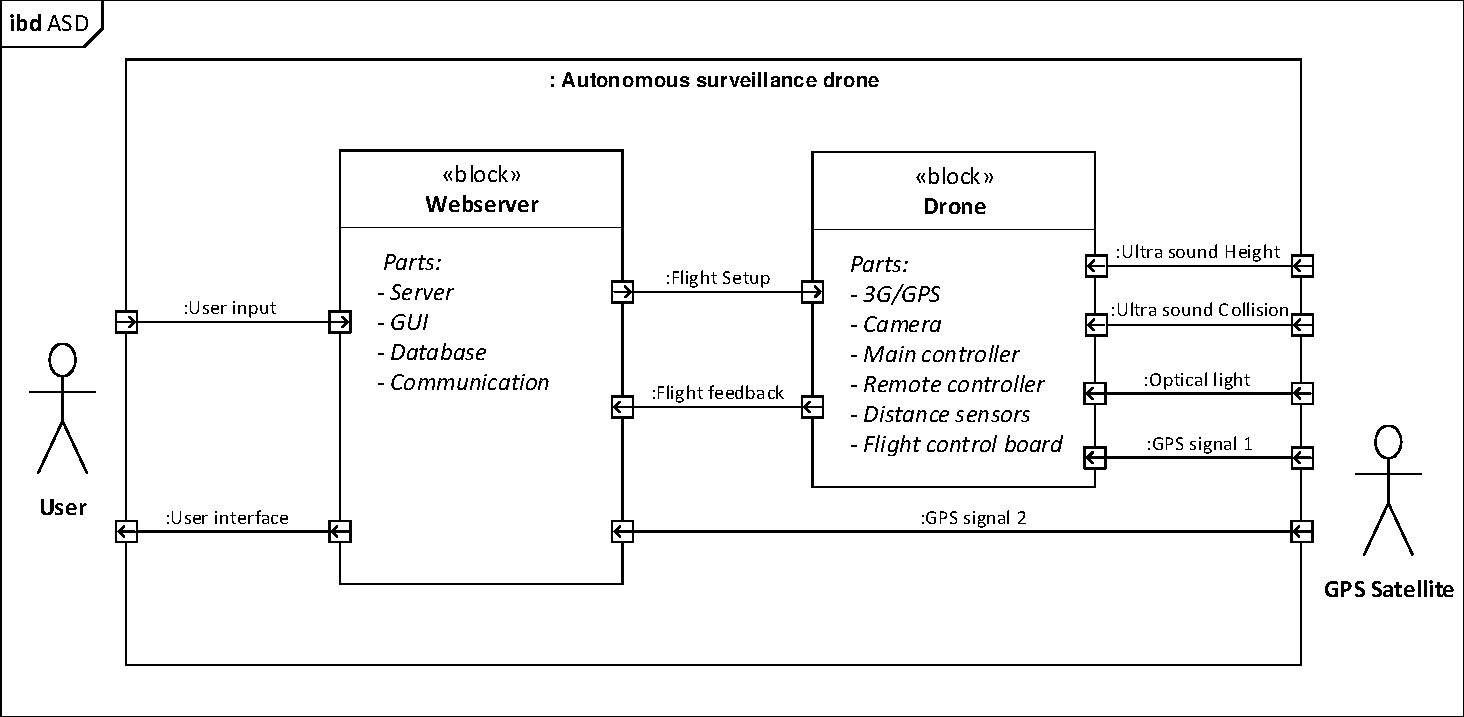
\includegraphics[width=1\textwidth]{Billeder/IBD/ibd1_overordnet.pdf}
\vspace{-1cm}
\caption{Ibd - ASD}
\label{fig:ibd_overordnet}
\end{figure}

\begin{table}[H]
	\centering
		\begin{tabular}{|p{2.6 cm}|p{4.9 cm}|p{2.5 cm}|p{2.5 cm}|} 
		\hline
			\textbf{Signal navn} 	& \textbf{Signal beskrivelse}		& \textbf{Out} 				& \textbf{In}     \\ \hline
			User input 			& Via \textit{webserver} opsætter \newline bruger ny eller undersøger tidligere flyvning & Bruger 		& Webserver.			    \\ \hline
			User interface 		& Via GUI kan bruger se hvad der sker i \textit{webserver}.	& Webserver.			& Bruger.				\\ \hline
			Flight setup		& Fra \textit{webserver} sendes \newline flyveopsætningen til dronen.	& Webserver.	& Dronen.	\\ \hline
			Flight feedback		& Informationer fra dronen \newline til \textit{webserver}.	& 	Dronen.		& Webserver.			    \\ \hline
			GPS signal 1		& GPS signal.	& GPS-satellit.			& Dronen.				\\ \hline
			GPS signal 2		& GPS signal.	& GPS-satellit.				& Webserver.	\\ \hline  
			Optical light		& Lys til at tage billeder.	& Drone \newline omgivelser.				& Drone.	\\ \hline 
			Ultra sound \newline Height		& Lydsignal reflekteres tilbage til ultralyds sensor.	& Drone \newline omgivelser.				& Drone.	\\ \hline 
			Ultra sound \newline Collision		& Lydsignal reflekteres tilbage til ultralyds sensor.	& Drone \newline omgivelser.				& Drone.	\\ \hline 
		\end{tabular}
	\caption{Forbindelser tilhørende: \textit{Ibd - ASD}}
	\label{tab:IBD1}
\end{table}

